%!TEX TS-program = xelatex 
%!TEX TS-options = -output-driver="xdvipdfmx -q -E"
%!TEX encoding = UTF-8 Unicode
%
%  my_title
%
%  Created by my_name on date.
%  Copyright (c) year. All rights reserved.
%

\documentclass[12pt]{article} 

% Definitions
\newcommand\mykeywords{color, illusion} 
\newcommand\myauthor{Mark Eli Kalderon} 
\newcommand\mytitle{Color Illusion}
\newcommand\mybib{Philosophy.bib}

% Packages
\usepackage{geometry} \geometry{a4paper} 
\usepackage{url}
\usepackage{txfonts}
\usepackage{color}
\definecolor{gray}{rgb}{0.459,0.438,0.471}
% \usepackage{setspace}
% \doublespace % Uncomment for doublespacing if necessary
\usepackage{epigraph} % optional

% XeTeX
\usepackage[cm-default]{fontspec}
\usepackage{xltxtra,xunicode}
\defaultfontfeatures{Scale=MatchLowercase,Mapping=tex-text}
\setmainfont{Palatino}
\setsansfont{Gill Sans}
\setmonofont{Inconsolata}

% Section Formatting
\usepackage[]{titlesec}
\titleformat{\section}[hang]{\fontsize{14}{14}\scshape}{\S{\thesection}}{.5em}{}{}
\titleformat{\subsection}[hang]{\fontsize{12}{12}\scshape}{\S{\thesubsection}}{.5em}{}{}
\titleformat{\subsubsection}[hang]{\fontsize{12}{12}\scshape}{\S{\thesubsubsection}}{.5em}{}{}

% Headers and Footers
\usepackage{fancyhdr}
\pagestyle{fancy}
\pagenumbering{arabic}
\lhead{\thepage}
\chead{}
\rhead{\itshape{\nouppercase{\leftmark}}}

% TODO List
\usepackage{color}
\usepackage{index} % use index package to create indices
\newindex{todo}{tod}{tnd}{TODO List} % start todo list
\newindex{fixme}{fix}{fnd}{FIXME List} % start fixme list
\newcommand{\todo}[1]{\textcolor{blue}{TODO: #1}\index[todo]{#1}} % macro for todo entries
\newcommand{\fixme}[1]{\textcolor{red}{FIXME: #1}\index[fixme]{#1}} % macro for fixme entries

% Bibliography
\usepackage[round]{natbib} 

% Title Information
\title{\mytitle} % For thanks comment this line and uncomment the line below
%\title{\mytitle\thanks{}}% 
\author{\myauthor} 
% \date{} % Leave blank for no date, comment out for most recent date

% PDF Stuff
\usepackage[plainpages=false, pdfpagelabels, bookmarksnumbered, backref, pdftitle={\mytitle}, pagebackref, pdfauthor={\myauthor}, pdfkeywords={\mykeywords}, xetex, dvipdfmx, colorlinks=true, citecolor=gray, linkcolor=gray, urlcolor=gray]{hyperref} 



%%% BEGIN DOCUMENT
\begin{document}

% Title Page
\maketitle
% \begin{abstract} % optional
% \end{abstract} 
\vskip 2em \hrule height 0.4pt \vskip 2em
% \epigraph{text of epigraph}{\textsc{author of epigraph}} % optional; make sure to uncomment \usepackage{epigraph}

% Layout Settings
\setlength{\parindent}{1em}

% Main Content

\section{Introduction} % (fold)
\label{sec:introduction}

I have lost my grip on what a color illusion is meant to be. Perhaps I have simply lost my grip---not an alternative to be ruled out in advance of inquiry. However, I believe that there is an alternative explanation. I have come to suspect that there is nothing answering to the philosopher's conception of illusion. That's not to say that there are no color experiences that might, with propriety, be described as illusory. There is a familiar genre of books illustrating optical illusions, many essentially involving chromatic phenomena. No charge of false advertising is leveled here. It is only a distinctively \emph{philosophical} conception of illusion whose claims are exaggerated. Or so I have, lately, come to suspect.

% section introduction (end)

\section{Benham's Disk} % (fold)
\label{sec:benham_s_disk}

Let's begin by considering an example of a color illusion often cited by philosophers---Benham's disk.

In 1894, an English toymaker, Charles Benham, devised a top adorned with a black and white pattern (see Figure~\ref{fig:benham}). Sold through Messrs. Newton and Co., an announcement of the ``Artificial Spectrum Top'' was published in \emph{Nature}:
\begin{quote}
	The top consists of a disc, one half of which is black, while the other half has twelve arcs of concentric circles drawn upon it. Each arc subtends an angle of forty-five degrees. In the first quadrant there are three such concentric arcs, in the next three more, and so on; the only difference being that the arcs are parts of circles of which the radii increase in arithmetical progression. Each quadrant thus contains a group of arcs differing in length from those of the other quadrants. The curious point is that when this disc is revolved, the impression of concentric circles of different colors is produced upon the retina. If the direction of rotation is reversed, the order of these tints is also reversed. \citep{Benham:1894kx}
\end{quote}
Specifically, if rotated clockwise, the innermost arcs form reddish rings, the next greenish rings, the next light blue rings, and the outermost arcs form violet rings. If rotated counterclockwise the pattern is reversed with the innermost arcs now forming violet rings and the outermost reddish rings. These apparent colors are puzzling. Each of the spinning arcs reflect light with the same spectral content and with equal average luminance. In advance of observing the spinning disk, then, one might reasonably expect the spinning arcs to appear as gray rings of equal brightness. The mysterious apparent colors of Benham's spinning disk are the ``subjective colors'' first described by \citep{Fechner:1838vn} (and, hence, are also sometimes described as ``Fechner-Benham colors''). The subjective colors produced by Benham's spinning disk are not completely understood; for a review of some of the color science see \citet{Campenhausen:1995yq}.

\begin{figure}[htbp]
	\centering
		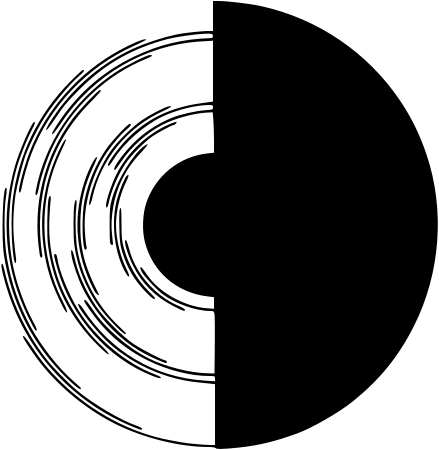
\includegraphics[scale=.5]{graphics/benhams_disk.jpg}
	\caption{Benham's Disk}
	\label{fig:benham}
\end{figure}

The subjective colors of the Benham disk are usually reckoned to be illusory. The surface of the disk is black and white. No part of the surface of the disk is reddish, or greenish, or light blue, or violet. So these apparent colors are merely apparent. In experiencing the reddish ring, we are perceiving something which is, in fact, not at all reddish. To that extent at least, the reddish appearance is \emph{illusory}. Similar reasoning holds for each of the subjective colors produced by the spinning disk.

\section{Pointillism and the Argument from Microscopes}\label{sec:pointillism_and_the_argument_from_microscopes} % (fold)

It would seem, then, that the subjective colors produced by the Benham disk are straightforward examples of color illusions as standardly conceived by philosophers. So what's the problem?

To bring out the problem, I want to compare the subjective colors produced by Benham's disks with two other chromatic phenomena. A proper understanding of these renders unsound the reasoning to the conclusion that the subjective colors produced by Benham's disk are illusory.

% section benham_s_disk (end)

\subsection{Pointillism}\label{sub:pointillism} % (fold)

Michel Eugène Chevreul, a French chemist appointed by Louis \textsc{xvii} as the director of the dye department of Manufacture Royale des Gobelins, upon receiving complaints that the black dyes they produced looked different when used alongside blue dye, investigated the matter and discovered the phenomena of simultaneous color contrast---that the appearance of a color can vary as the color of the surrounding scene varies. \citet{Chevreul:1855kx} reported his findings in his book, \emph{The Principles of Harmony and Contrast of Colours and Their Application to the Arts}, a book that influenced the work of the French painter Georges-Pierre Seurat. Fascinated by the appearance of a color being influenced by adjacent colors, Seurat eventually paints the pointillist masterpiece, “Un dimanche après-midi à l'Île de la Grande Jatte” in 1884--6. Using only primary unblended pigments, including the newly available zinc yellow, these were distributed in small dots across the surface of the canvas giving rise to the appearance, at an appropriate distance, of a differently colored scene of Parisian suburbanites relaxing by the river Seine.

Imagine, then, if you will, viewing a minimalist painting in a gallery. From your current vantage point, the surface of the painting appears a uniform if luminous green. Closer inspection is revealing, however. As you move in for a closer look, the painting is discovered to be not only minimalist, but pointillist. The luminous green appearance of the surface was achieved by painstakingly painting minute yellow and blue dots across the surface. In fact no part of the surface of the painting is green---every part of the surface is either yellow or blue. One might be tempted to conclude that the green appearance of the painting was illusory. If no part of the surface of the painting is green, then how could the green appearance be veridical? 

It would seem that we have here reasoning that straightforwardly parallel's the reasoning that convicted the subjective colors of being illusory. However, the reasoning in this intermediary case is fallacious as Hilbert's \citeyear[chapter 2]{Hilbert:1987jq}, discussion of Berkeley's \citeyear{Berkeley:1734fk} argument from microscopes reveals.

% subsection pointillism (end)

\subsection{The Argument from Microscopes}\label{sub:the_argument_from_microscopes} % (fold)

In arguing against the claim that ``the colors which we see exist in external bodies'', Berkeley presents the argument from microscopes:
\begin{quote}
	PHILONUS: `Apparent' colors you call them? How shall we distinguish these apparent colors from real?\\
	HYLAS: Very easily. They are to be thought apparent which appearing only at a distance, vanish upon a nearer approach.\\
	PHILONUS: And those, I suppose, are to be thought real which are discovered by the most near and exact survey.\\
	HYLAS: By a microscope, doubtless.\\
	PHILONUS: But a microscope often discovers colors in an object different from those perceived by the unassisted sight. And, in case we had microscopes mangnifying to any assigned degree, it is certain that no object whatsoever, viewed through them, would appear in the same color which it exhibits to the naked eye.\\
	HYLAS: And what will you conclude from all this? You cannot argue that there are really and naturally no colors on objects because by artificial managements they may be altered or made to vanish.\\
	PHILONUS: I think it may be evidently concluded from your own concessions that all the colors we see with our naked eyes are only apparent as those on the clouds, since they vanish upon a more close and accurate inspection which is afforded us by a microscope.
\end{quote}
The conclusion of this argument is that either the appearance of the object to the naked eye or its appearance through a microscope is illusory. But from here, all that is required to reach the claim that all color is apparent is the application of classic Pyrrhonian reasoning---justify which of these vantage points affords us knowledge of the true colors of things or give up the claim that colors inhere in external objects. For if the naked eye and the microscope each have equal claim to affording us knowledge of the colors of external objects, then neither do.

\citet{Hilbert:1987jq} adapts a version of the argument from microscopes due to \citet{Marc-Wogau:1968kx}. A drop of fresh blood looks uniformly red to the naked eye. However, as Locke observed, blood, when viewed under a microscope, looks ``pellucid''---it looks partly red and partly transparent. These appearances seemingly conflict given the plausibility of the following exclusion principle---that nothing can be uniformly red all over and partly red and partly transparent. If the conflict is genuine, then the Berkelean conclusion follows---that either the appearance of the drop of blood to the naked eye is illusory or the blood's appearance through the microscope is illusory. 

However, as \citet{Hilbert:1987jq} observes, no genuine conflict is generated. It is not that the exclusion principle is false, only that it has no present application. There is no one thing that appears red all over and partly red and partly transparent. A drop of blood may look red to the naked eye, but we do not see the drop of blood under the microscope; we see only a part of it. To a generate a conflict in appearance, the argument from microscopes needs to appeal to a different principle. Specifically, if what is viewed under the microscope is a part of the drop of blood, to generate a conflict we would need the assumption that if something is colored, then all of its parts must have the same color. We would need to assume that color is \emph{dissective} in something like Goodman's sense of the term:
\begin{quote}
	A one-place predicate is said to be \emph{dissective} if it is satisfied by every part of every individual that satisfies it. Since every part of everything that is smaller than Utah is also smaller than Utah, the predicate ``is smaller than Utah'' is dissective. \citep[53]{Goodman:1951ww}
\end{quote}
If color is dissective, then if the drop of blood is red, then so must all of its parts. Since the part of the blood viewed under a microscope is partly red and partly transparent, then either the appearance of the drop of blood is illusory or the blood's appearance when viewed under a microscope is illusory.

Are colors genuinely dissective? Goodman himself denies that they are:
\begin{quote}
	Different perceptible parts of any object may be differently colored even if the object itself is uniform and unvarying in color. This is no more paradoxical than the fact that a single object contains spatiotemporally different parts. As the self-identical object is a function of its parts, so the single unchanging color of the object is a function of the colors of its parts. The nature and interrelation of the lesser elements that make up the whole determine what kind of thing the whole is: the kind and arrangement of the colors exhibited by these various parts determine what color the whole is said to have. \citep[130]{Goodman:1951ww}
\end{quote}
In tacitly assuming that color is dissective, Berkeley seems to be assuming that once we have seen an object to be a certain color, we have seen all that there is to see about its color, including the color of its parts. This, however, flies in the face of a modest and attractive picture of perception as providing only partial perspective on the material environment. If perception is partial, then what is seen depends not only on what there is to see, but on the visual sensibility of the perceiver and the circumstances of perception. In seeing the scene before us, the scene is presented to our partial perspective on that scene. The visible aspects of the scene is not wholly determined by any given perception of it---other partial perspectives on that scene may reveal further visible aspects. It is this commitment to perception as providing a partial perspective on the material environment, that leads Hilbert to describe, Berkeley's argument from microscopes as committing the ``fallacy of total information''. In effect, Berkeley fallaciously reasons from our failing to perceive that the drop of blood has transparent parts, to our perceiving that no part of the blood is transparent.

A weaker principle is consistent with perception being partial:
\begin{quote}
	If from a particular partial perspective, as determined by the visual sensibility of the perceiver and the circumstances of perception, an object appears to be a uniform color, then all of the parts of that object that are visible from that partial perspective have that color.
\end{quote}
However, this weaker principle is insufficient to generate a conflict in appearance. The ``pellucid'' parts of the blood are not visible to the naked eye. And if no conflict is generated, then the Berkelean conclusion fails to follow.

% subsection the_argument_from_microscopes (end)

\subsection{Pointillism Revisited}\label{sub:pointillism_revisited} % (fold)

Consider again viewing the minimalist painting in a gallery. From your current vantage point, the surface of the painting appears a uniform if luminous green. When viewed more closely, however, the painting is discovered to be not only minimalist, but pointillist. The luminous green appearance was achieved by painting minute yellow and blue dots across the surface of the canvas. When viewed more closely, then, the canvas appears partly yellow and partly blue. Are these appearances in conflict such that we must convict one or the other of these appearances as being illusory? If perception is partial, then there is no conflict. From the fact that, from a particular perspective, the painting appears uniformly green, all that follows is that all of the parts of the painting \emph{visible from that partial perspective} are green. As the minute blue and yellow parts are not visible from that perspective, no conflict is generated.

An unwarranted atomism may be responsible for a lingering sense that the green appearance of the picture is illusory. This atomism is at work in Armstrong's version of the argument from microscopes:
\begin{quote}
	A microscope is deployed bit by bit over the whole of an area easily visible to the naked eye. A certain colour picture of the area could be built up---it could be literally pictured on some much larger area---which will, in general, be incompatible with the colour appearances presented to the naked eye. Thus a drop of blood looks red all over to the naked eye, but a colour picture of the same drop obtained by deploying a microscope over the whole surface of the drop would not contain very much red. \citep[108]{Armstrong:1968nx}
\end{quote}
Armstrong's idea is that the color of a whole is the color obtained by making a map of the color of its parts. In effect, the color of the whole is identified with the aggregate of the colors of the minimum visibilia. There is a lot that may be questioned here. Why has Berkeley's Pyrronian crisis between mites and men been resolved in favor of mites? Do minimum visibilia even exist? Set aside such questions for the moment and consider the application of Armstrong's idea to the case of the pointillist painting. If the color of the whole is the aggregate of the color of the minimum visibilia, then since none of the minimum visibilia are green, the green appearance of the painting when viewed from a certain distance is illusory.

It may be true, as Goodman suggests, that the color of a whole is a function of the color of its parts, but this does not entail the particular function that Armstrong appeals to. Moreover, the principle that Armstrong appeals to does not hold generally of perceptible properties. The shape of a whole need not be the shape of its parts---even its minimally visible parts if such there be. The real problem for Armstrong's atomism is that it is inconsistent with perception affording a partial perspective on the material environment. If perception is partial, then an object need not display all of its colors from an given perspective. Even if it is possible to view the entire surface of the drop of blood through a microscope, the drop of blood may not reveal all of its colors to that perspective. Similarly, even it is possible to view the entire surface of the painting and see it as composed of blue and yellow dots, the painting may not reveal all of its colors from that perspective. If perception provides a partial perspective on the material environment, the green appearance of the painting, when viewed from a certain distance, is not illusory. 

% subsection pointillism_revisited (end)

% section pointillism_and_the_argument_from_microscopes (end)

% Bibligography
\bibliographystyle{plainnat} 
\bibliography{Philosophy.bib} 

\end{document}
